\documentclass[letterpaper,12pt]{article}

\usepackage{threeparttable}
\usepackage{geometry}
\geometry{letterpaper,tmargin=1in,bmargin=1in,lmargin=1.0in,rmargin=1.0in}
\usepackage[format=hang,font=normalsize,labelfont=bf]{caption}
\usepackage{amsmath}
\usepackage{multirow}
\usepackage{xcolor}
\usepackage{array}
\usepackage{delarray}
\usepackage{amssymb}
\usepackage{amsthm}
\usepackage{lscape}
\usepackage{natbib}
\usepackage{setspace}
\usepackage{float,color}
\usepackage[pdftex]{graphicx}
\usepackage{listings}
\lstset{basicstyle=\footnotesize\ttfamily, language=Python, showstringspaces=false}

\lstset{frame=single,
  language=Python,
  showstringspaces=false,
  columns=flexible,
  basicstyle={\small\ttfamily},
  numbers=none,
  breaklines=true,
  breakatwhitespace=true
  tabsize=3
}

\usepackage{pdfsync}
\usepackage{booktabs}
\usepackage{verbatim}
\usepackage{placeins}
\usepackage{geometry}
\usepackage{pdflscape}
\synctex=1
\usepackage{hyperref}
\hypersetup{colorlinks,linkcolor=red,urlcolor=blue,citecolor=red}
\usepackage{bm}


\theoremstyle{definition}
\newtheorem{theorem}{Theorem}
\newtheorem{acknowledgement}[theorem]{Acknowledgement}
\newtheorem{algorithm}[theorem]{Algorithm}
\newtheorem{axiom}[theorem]{Axiom}
\newtheorem{case}[theorem]{Case}
\newtheorem{claim}[theorem]{Claim}
\newtheorem{conclusion}[theorem]{Conclusion}
\newtheorem{condition}[theorem]{Condition}
\newtheorem{conjecture}[theorem]{Conjecture}
\newtheorem{corollary}[theorem]{Corollary}
\newtheorem{criterion}[theorem]{Criterion}
\newtheorem{definition}{Definition}  % Number definitions on their own
\newtheorem{derivation}{Derivation}  % Number derivations on their own
\newtheorem{example}[theorem]{Example}
\newtheorem{exercise}[theorem]{Exercise}
\newtheorem{lemma}[theorem]{Lemma}
\newtheorem{notation}[theorem]{Notation}
\newtheorem{problem}[theorem]{Problem}
\newtheorem{proposition}{Proposition}  % Number propositions on their own
\newtheorem*{proposition*}{Proposition}  % Non-numbered proposition
\newtheorem{remark}[theorem]{Remark}
\newtheorem{solution}[theorem]{Solution}
\newtheorem{summary}[theorem]{Summary}
\bibliographystyle{aer}
\newcommand\ve{\varepsilon}
%\renewcommand\theenumi{\roman{enumi}}
\newcommand\norm[1]{\left\lVert#1\right\rVert}

\begin{document}

\begin{titlepage}
\title{The Economic Costs of Public Health Spending Cuts: HIV/AIDS and Tuberculosis in South Africa}
\date{\today}
\author{\href{http://jasondebacker.com/}{Jason DeBacker}\thanks{University of South Carolina, Darla Moore School of Business, Department of Economics, \href{mailto:jason.debacker@moore.sc.edu}{jason.debacker@moore.sc.edu}.}\and \href{https://sites.google.com/site/rickecon}{Richard W. Evans}\thanks{\href{https://abundance.institute/}{Abundance Institute}, \href{mailto:rick@abundance.institute}{rick@abundance.institute}.}\and {Marcelo T. LaFleur}\thanks{{United Nations Department of Economic Social Affairs}, \href{mailto:lafleurm@un.org}{lafleurm@un.org}. The views and opinions expressed herein are the author's and do not necessarily reflect those of the United Nations Secretariat.}}
\maketitle
\vspace{-2mm}
\begin{abstract}
\small{Our broad research question is to study the individual and macroeconomic effects of public health spending. Reductions in US foreign aid are expected to have significant public health impacts, which will generate macroeconomic impacts. We estimate the economic costs of these reductions in terms of lost health, population, and productivity for South Africa. We study South Africa because it is the country with the highest number of people living with HIV/AIDS. We find that the reductions in foreign aid and expected significant increases in disease and premature death will have large and negative impacts on the South African economy. In our preferred specification, the costs of US aid cuts to South Africa exceed \$3.1 trillion dollars in net present value, reducing economic output by more than 3.5\%. These simulations provide a quantititive estimate of the return on investment of public health spending.}

\vspace{10mm}

\noindent\textit{keywords:}\: public health, demographics, general equilibrium, productivity, South Africa

\vspace{10mm}

\noindent\textit{JEL classification:} C68, E24, E37, I15, J11, J17, J24


\end{abstract}
\thispagestyle{empty}
\end{titlepage}


\begin{spacing}{1.5}

\pagenumbering{arabic}

\newpage

\section{Introduction}\label{SecIntro}

South Africa has carried one of the world's heaviest HIV/AIDS burdens for over two decades. HIV prevalence has remained among the highest globally, with 17.1\% of adults infected with the virus in 2023 and a total of 7.7 million people living with HIV \citep{UNAIDSData2024}. The dual burden of HIV and tuberculosis (TB), still the world's deadliest infectious disease, has compounded the country's health crisis.

This persistent disease burden has generated far-reaching economic and social consequences. As of 2023, 5.9 million people between the ages of 15 and 49 were HIV-positive, and South Africa recorded the highest absolute labor income losses globally due to HIV-related illness and mortality \citep{ILO2018}. These effects are not confined to the formal labor market. Unpaid care burdens, disruptions to education, and lower household productivity compound the long-term developmental cost. The cumulative strain on human capital, social protection systems, and economic growth has become a defining feature of South Africa's development trajectory.

Despite these challenges, the large-scale expansion of antiretroviral therapy (ART) for treating HIV has dramatically improved survival and reduced transmission. By 2023, approximately 77\% of HIV-positive individuals were receiving ART, reflecting one of the highest coverage rates in the region \citep{UNAIDSData2024}. This progress was made possible largely through sustained external financing and partnerships that supported clinical infrastructure, drug procurement, and health workforce training. South Africa's response to HIV and TB has thus become structurally dependent on international support. Continued access to external funding has been essential to maintaining treatment programs, expanding prevention efforts, and preserving health system resilience.

South Africa's reliance also introduces vulnerabilities in the face of shifting global aid priorities. The outsized role of the United States in financing HIV/AIDS programs in low- and middle-income countries, particularly through the President's Emergency Plan for AIDS Relief (PEPFAR), results in South Africa being especially affected by US aid policy. According to the Institute for Health Metrics and Evaluation report \citep{FGH2023}, total US development assistance for health (DAH) rose from \$19.1 billion in 2021 to approximately \$20.6 billion in 2023—a 7.8\% increase. US funding for HIV/AIDS globally accounted for nearly \$8.6 billion of that total in 2023. South Africa is among the largest absolute recipients of this assistance, receiving \$462 million in 2023 that supports prevention programs, treatment coverage, public health infrastructure, and the training of medical personnel. Though countries such as Eswatini and Lesotho receive more funding per capita, the scale of South Africa's epidemic and population has made US support an indispensable foundation of its national HIV response.

In early 2025, the US government abruptly halted all USAID health disbursements, terminating more than 5,800 out of 6,300 contracts and grants globally in previously obligated commitments \citep{Cohen2025}. The fallout was immediate. The Joint United Nations Programme on HIV and AIDS (UNAIDS) lost nearly half its budget, clinics suspended services, and millions faced interruptions in care. In South Africa, public health leaders warned of a collapse in ART delivery systems, re-emergence of opportunistic infections, and surges in preventable deaths. The World Health Organization simultaneously issued an alert on disruptions to TB services, calling for urgent global action.

The human toll of this withdrawal is projected to be devastating. \citet{KS2025} estimate that the complete elimination of US global health funding could result in as many as 3.3 million excess deaths worldwide each year, with HIV/AIDS accounting for the majority of these losses. \citet{Gandhi2025} estimate that the cessation of PEPFAR funding could lead to up to 2.9 million additional HIV-related deaths over a ten-year period under the most severe scenario. \Citet{Brink2025} present an even more severe estimate in the worst case scenario that as many as 2.9 million people could die from HIV/AIDS in low- and middle-income countries over the next five years.

For South Africa, the various sources estimate excess deaths from HIV alone could amount anywhere from 14,000 to 192,000 annually, depending on how much US funding is cancelled and how much additional domestic funding is used to offset this loss. In addition to the direct loss of life, the increased disease burden resulting from disrupted treatment is expected to increase absenteeism and reduce labor productivity. These illness-related work absences can significantly lower effective labor supply \citep{Keogh2024,Panda2024}. These estimates highlight the dimensions and scale of the crisis and provide the basis for our economic simulation.

Our broad research agenda is to quantify the return on investment to public health initiatives that influence demographic dynamics through mortality rates and fertility rates and human welfare and labor productivity.\footnote{See \citet{DeBackerEtAl:2025}, \citet{RomanniEtAl:2025}, and \citet{RomanniEtAl:forthcoming} for research using this approach to study the effect of medical breakthroughs on individual and macroeconomic outcomes in the United States.} In this paper, we quantify the macroeconomic impact of US aid withdrawal on South Africa using an overlapping generations model calibrated to match features of the South African economy, including detailed demographics, labor market participation, fiscal capacity, and international capital flows. We use the excess mortality scenarios derived from recent projections by \citet{Brink2025}, \citet{Gandhi2025}, and by \citet{KS2025}, and expected changes to labor productivity associated with the higher disease burden \citep{Keogh2024,Panda2024}. In our framework, higher mortality and increased illness-related disutility of labor lead to reductions in labor supply, human capital, and long-run output.

By simulating these scenarios, this paper contributes to understanding the long-run economic costs of disease and the structural fragility of health systems that are highly dependent on external financing. Our findings highlight not only the human toll of abrupt aid cessation but also its deep implications for future macroeconomic performance and national development.


\section{Methodology}\label{SecMethod}

We estimate the macroeconomic effects of increased disease burden using the OG-ZAF macroeconomic model.\footnote{OG-ZAF is an open source large scale dynamic general equilibrium overlapping generations model of the South African macroeconomy. Documentation for OG-ZAF is available at \href{https://eapd-drb.github.io/OG-ZAF}{https://eapd-drb.github.io/OG-ZAF}. And documentation for the core engine OG-Core is available at \href{https://pslmodels.github.io/OG-Core}{https://pslmodels.github.io/OG-Core}.} OG-ZAF is a dynamic overlapping generations general equilibrium model calibrated to the demographic dynamics, economic parameters, and fiscal system of South Africa. It includes explicit modeling of household and firm behavior, government transfers and taxes, and age-specific labor supply and mortality rates. One of the key features of this modeling framework is its ability to capture both the direct and indirect effects of disease on the economy. The direct effects of disease include reductions in labor supply and productivity due to increased mortality and morbidity. The indirect effects include changes in capital accumulation, government budgets, and market prices, which will in turn affect labor supply and the overall economy.

We introduce exogenous shocks to mortality and productivity to reflect the effects of an abrupt reduction in external health financing. These shocks are implemented as changes to the age-specific mortality rates and labor disutility parameters in the model, capturing the consequences of untreated or poorly managed HIV and tuberculosis.

Our analysis is based on epidemiological projections of annual mortality increases following the abrupt cessation of PEPFAR funding. We draw on three independent estimates, each assuming full withdrawal of support without replacement funds from domestic sources (mitigation): \citet{Brink2025} (98,350 annual excess deaths), \citet{Gandhi2025} (132,600 deaths), and \citet{KS2025} (192,212 deaths). These estimates define our \textit{low}, \textit{mediumn}, and \textit{high} mortality scenarios, respectively. These inputs are described in detail below.

The resulting demographic and productivity shocks are introduced into the model, with a transition to higher mortality rates over the 2025-2030 period, but with an immediate increase the disutility of labor. This parameterization captures the nature of disease dynamics, where disruptions to treatment have rapid effects on worker absenteeism and labor supply, even as mortality effects accumulate more gradually.


\subsection{Epidemiological Scenarios}

\citet{Brink2025} estimate the expected increase in HIV-related mortality across 36 PEPFAR-supported countries by combining funding reduction scenarios with empirical elasticities derived from historical changes in treatment coverage and mortality. Their results show a sharp gradient in cumulative excess deaths from 2025 to 2030, depending on the scenario. In more benign scenarios there are few additional deaths. In more severe scenarios, where PEPFAR is discontinued, the projected excess mortality over the five-year period reaches 282,950 with mitigation efforts, and 491,750 without mitigation—averaging 56,590 and 98,350 additional deaths per year, respectively. We use this latter figure of 98,350 additional deaths per year as our \textit{low excess deaths scenario}. Despite this being the upper bound of the \citet{Brink2025} excess death estimates, this is the lowest estimate of the three studies we consider.

\citet{Gandhi2025} model clinical and economic outcomes under three scenarios of PEPFAR funding in 2024: full support, partial support, and complete withdrawal. Using the CEPAC-International microsimulation model,\footnote{See \href{https://mpec.massgeneral.org/cepac-model}{https://mpec.massgeneral.org/cepac-model}.} they project changes in HIV incidence, treatment coverage, and AIDS-related mortality in South Africa. The model tracks disease progression, care engagement, and mortality for both people with HIV and those at risk. Importantly, they also consider the effects of funding cuts on testing capacity, re-engagement in care, and prevention services. Under a scenario of complete withdrawal, they estimate as many as 1.3 million excess deaths over ten years in South Africa, relative to full funding, or 132,600 annual deaths. We use this estimate of 132,600 annual excess deaths as our \textit{medium excess deaths scenario}.

\citet{KS2025} estimate the lives saved by US foreign aid through both gross and net approaches. For HIV/AIDS, their gross estimate is based on the number of individuals receiving PEPFAR-funded antiretroviral therapy, combined with survival rates for untreated HIV to calculate an annualized total of 1.6 million lives saved.\footnote{The authors suggest this estimate is biased by the presence of small countries with high HIV prevalence.} Their net estimate relies on a differences-in-differences analysis which compares adult mortality trends in PEPFAR focus countries to non-PEPFAR recipient control countries. This analysis suggests that PEPFAR reduced all-cause mortality by roughly three deaths per 1,000 adults annually. Applying this to total US global HIV/AIDS aid yields an upper-bound estimate of nearly 3 million deaths averted per year, though the authors note this may overstate the true effect. For South Africa the authors estimate that 192,212 lives are saved each year due to US funding. We use this estimate as our upper-bound of expected lives lost due to the cancellation of US health aid, or the \textit{high excess deaths scenario}.

Figure \ref{fig:cumDeaths} shows the cumulative excess deaths in South Africa over the simulation horizon for each of these scenarios. The low excess death scenario is shown in blue, while the middle and high scenarios are shown in red and green, respectively.

\begin{figure}[H]
    \caption{Forecasted cumulative excess deaths in South Africa from US aid cuts}
    \label{fig:cumDeaths}
    \centering
    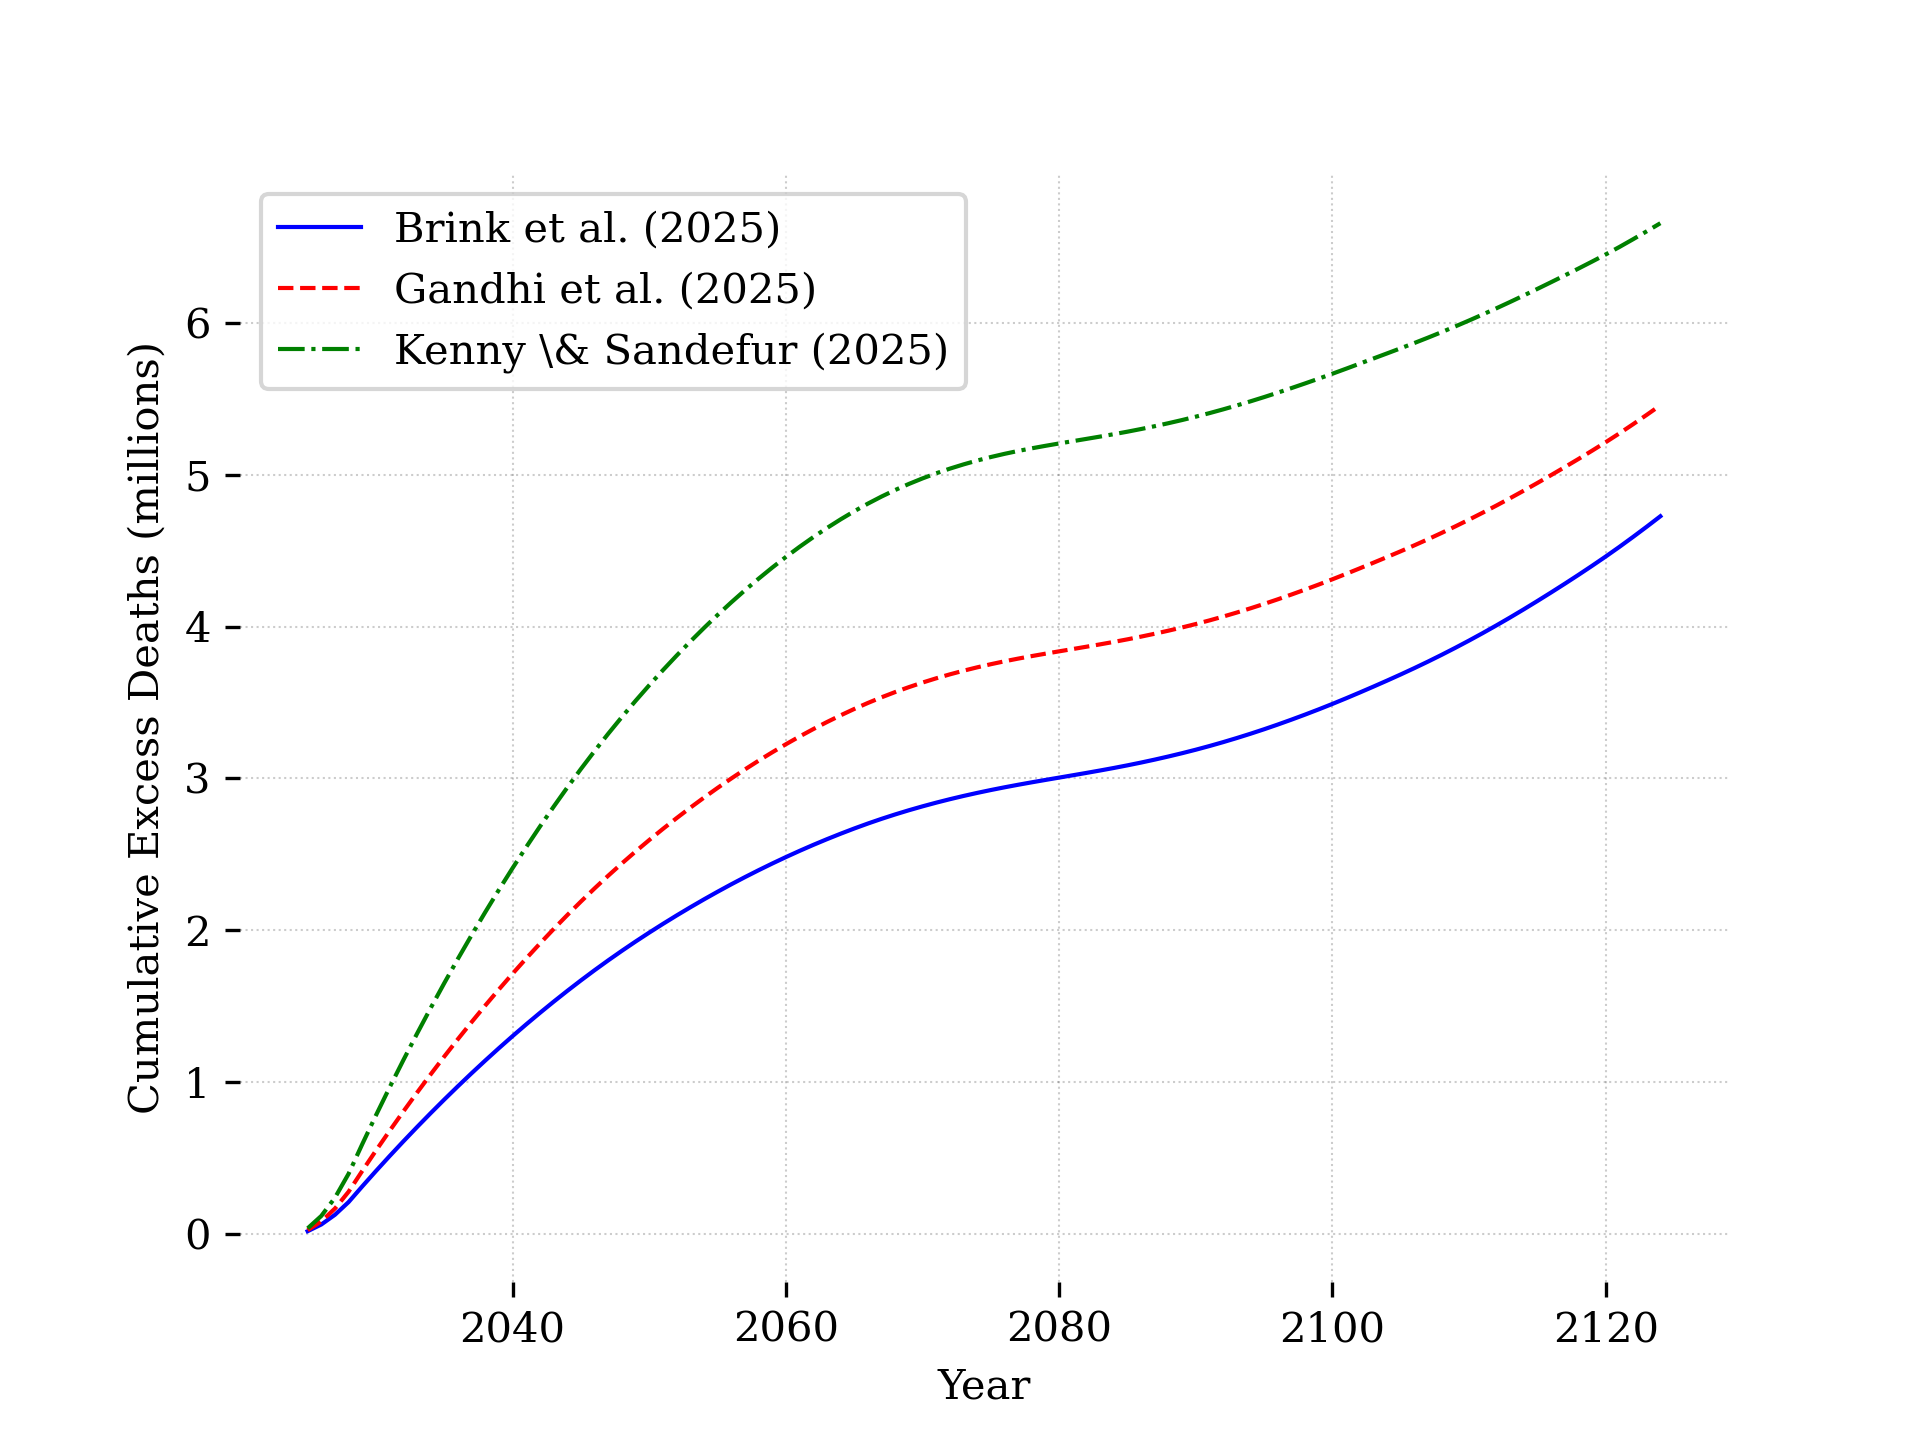
\includegraphics[scale=0.75]{./tables_figures/cumulative_excess_deaths.png}
\end{figure}

These estimates of excess deaths are mapped into the model through changes in the age-specific mortality rates. Specifically, we begin with current age-specific mortality rates as reported by the United Nations World Population Prospects 2024 \citep{UN2024}. We assume that these South African mortality rates by age are the mortality rates that would exist if there were no change in US aid to South Africa (blue line in Figure \ref{fig:Mortality}). We then apply a percentage adjustment to the mortality rates at each age to match the forecasts of excess deaths under each scenario. Figure \ref{fig:Mortality} shows increased mortality rates resulting from our low (red dashed line), medium (green dashed line) and high (teal dotted line) excess death scenarios for each age group in 2025.


\begin{figure}[H]
    \caption{South African mortality rates by age with and without aid}
    \label{fig:Mortality}
    \centering
    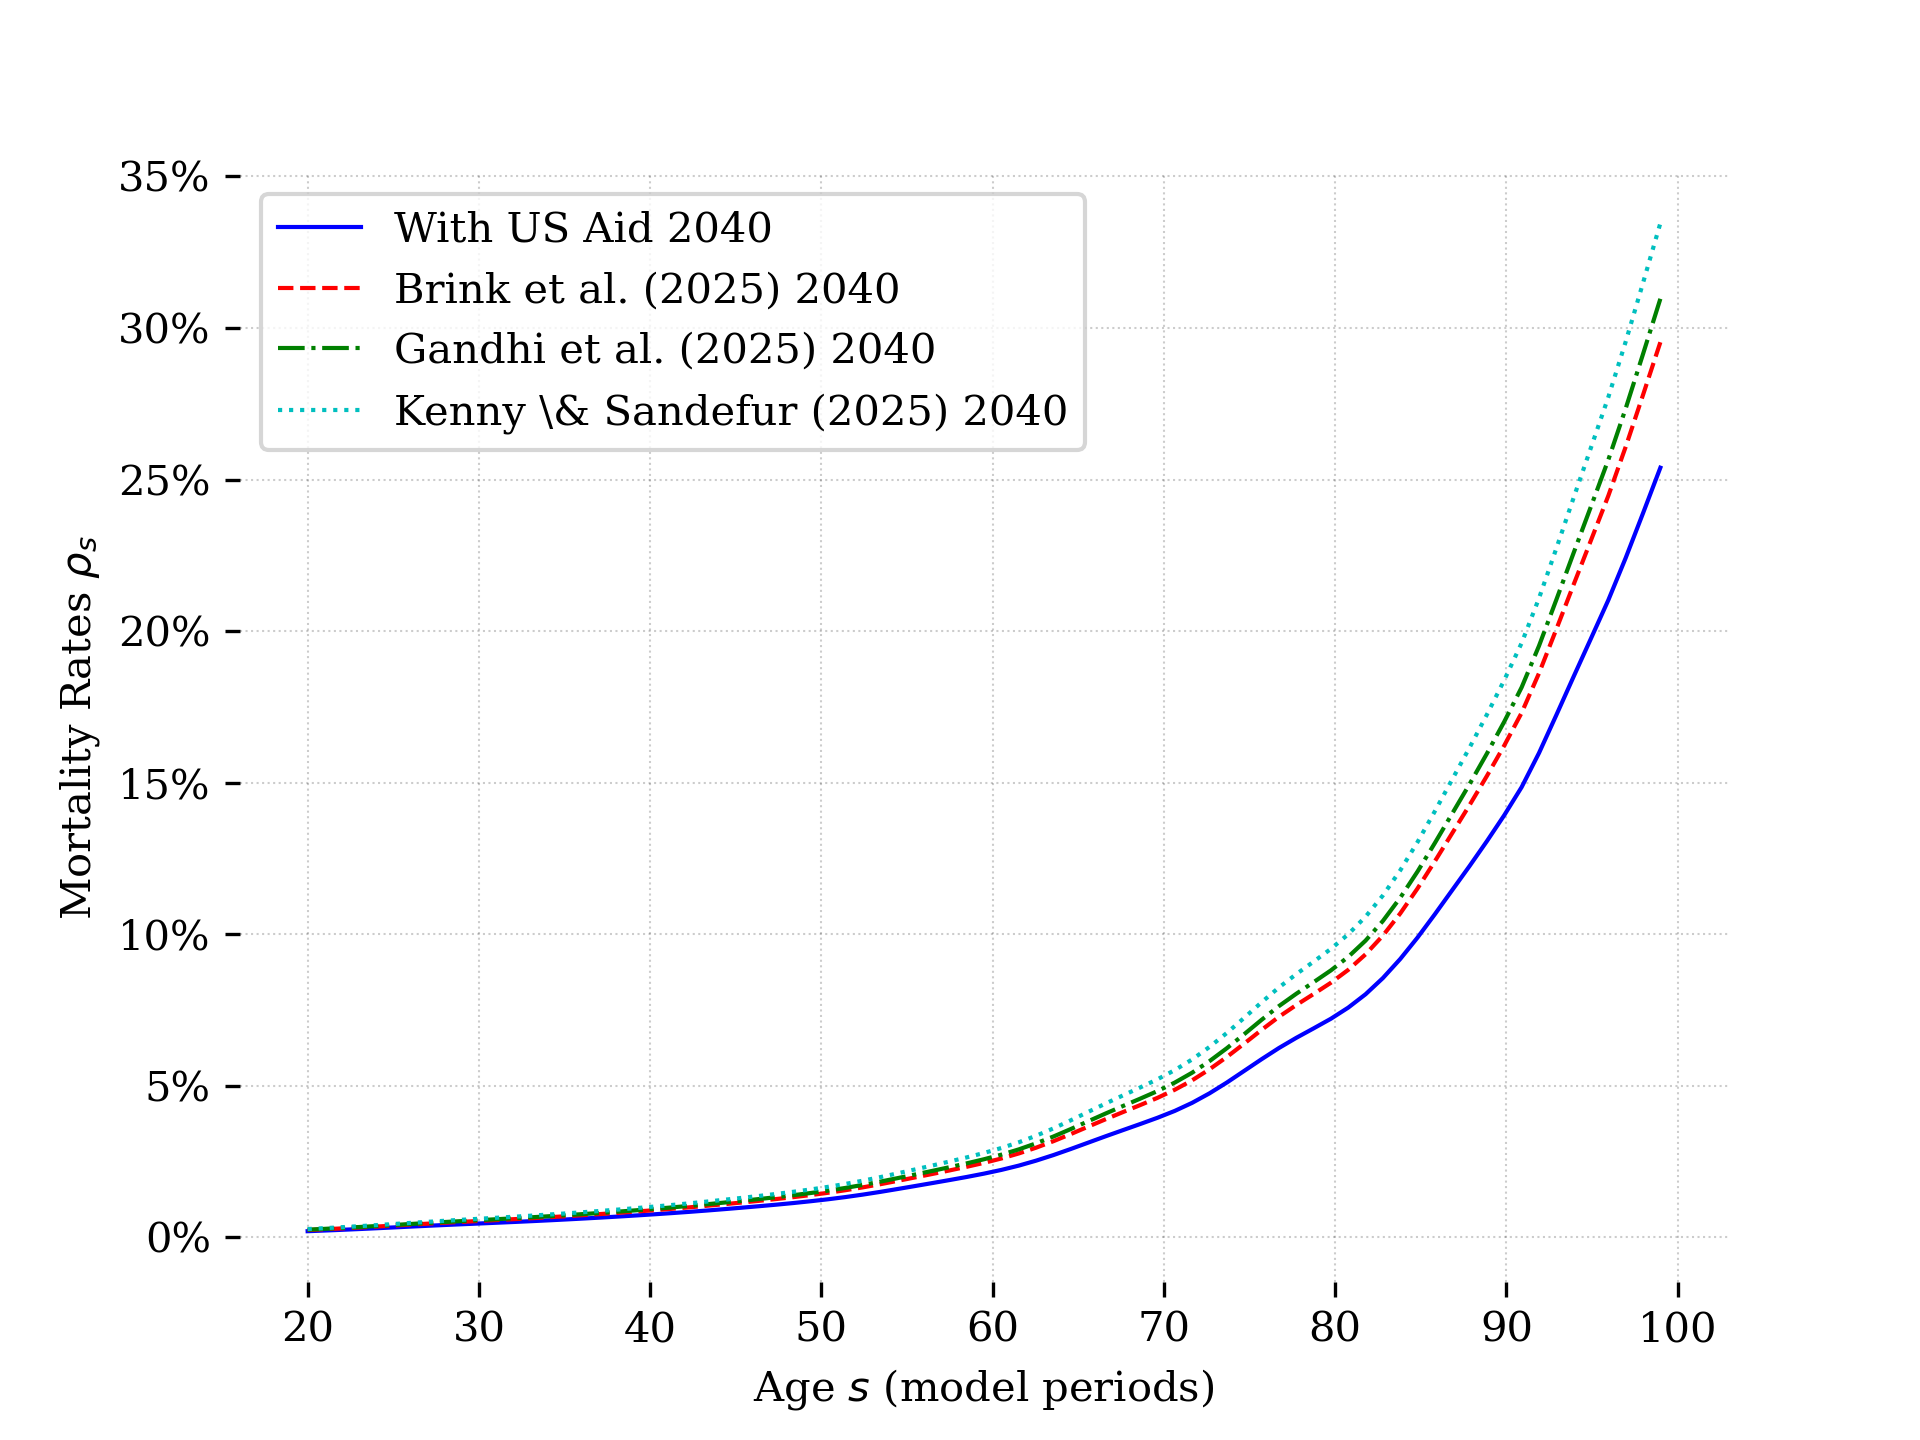
\includegraphics[scale=0.75]{./tables_figures/mortality_rates.png}
\end{figure}


% The population distribution is affected by the changes in mortality rates:
% \begin{figure}[H]
%     \caption{The population distribution with and without aid}
%     \centering
%     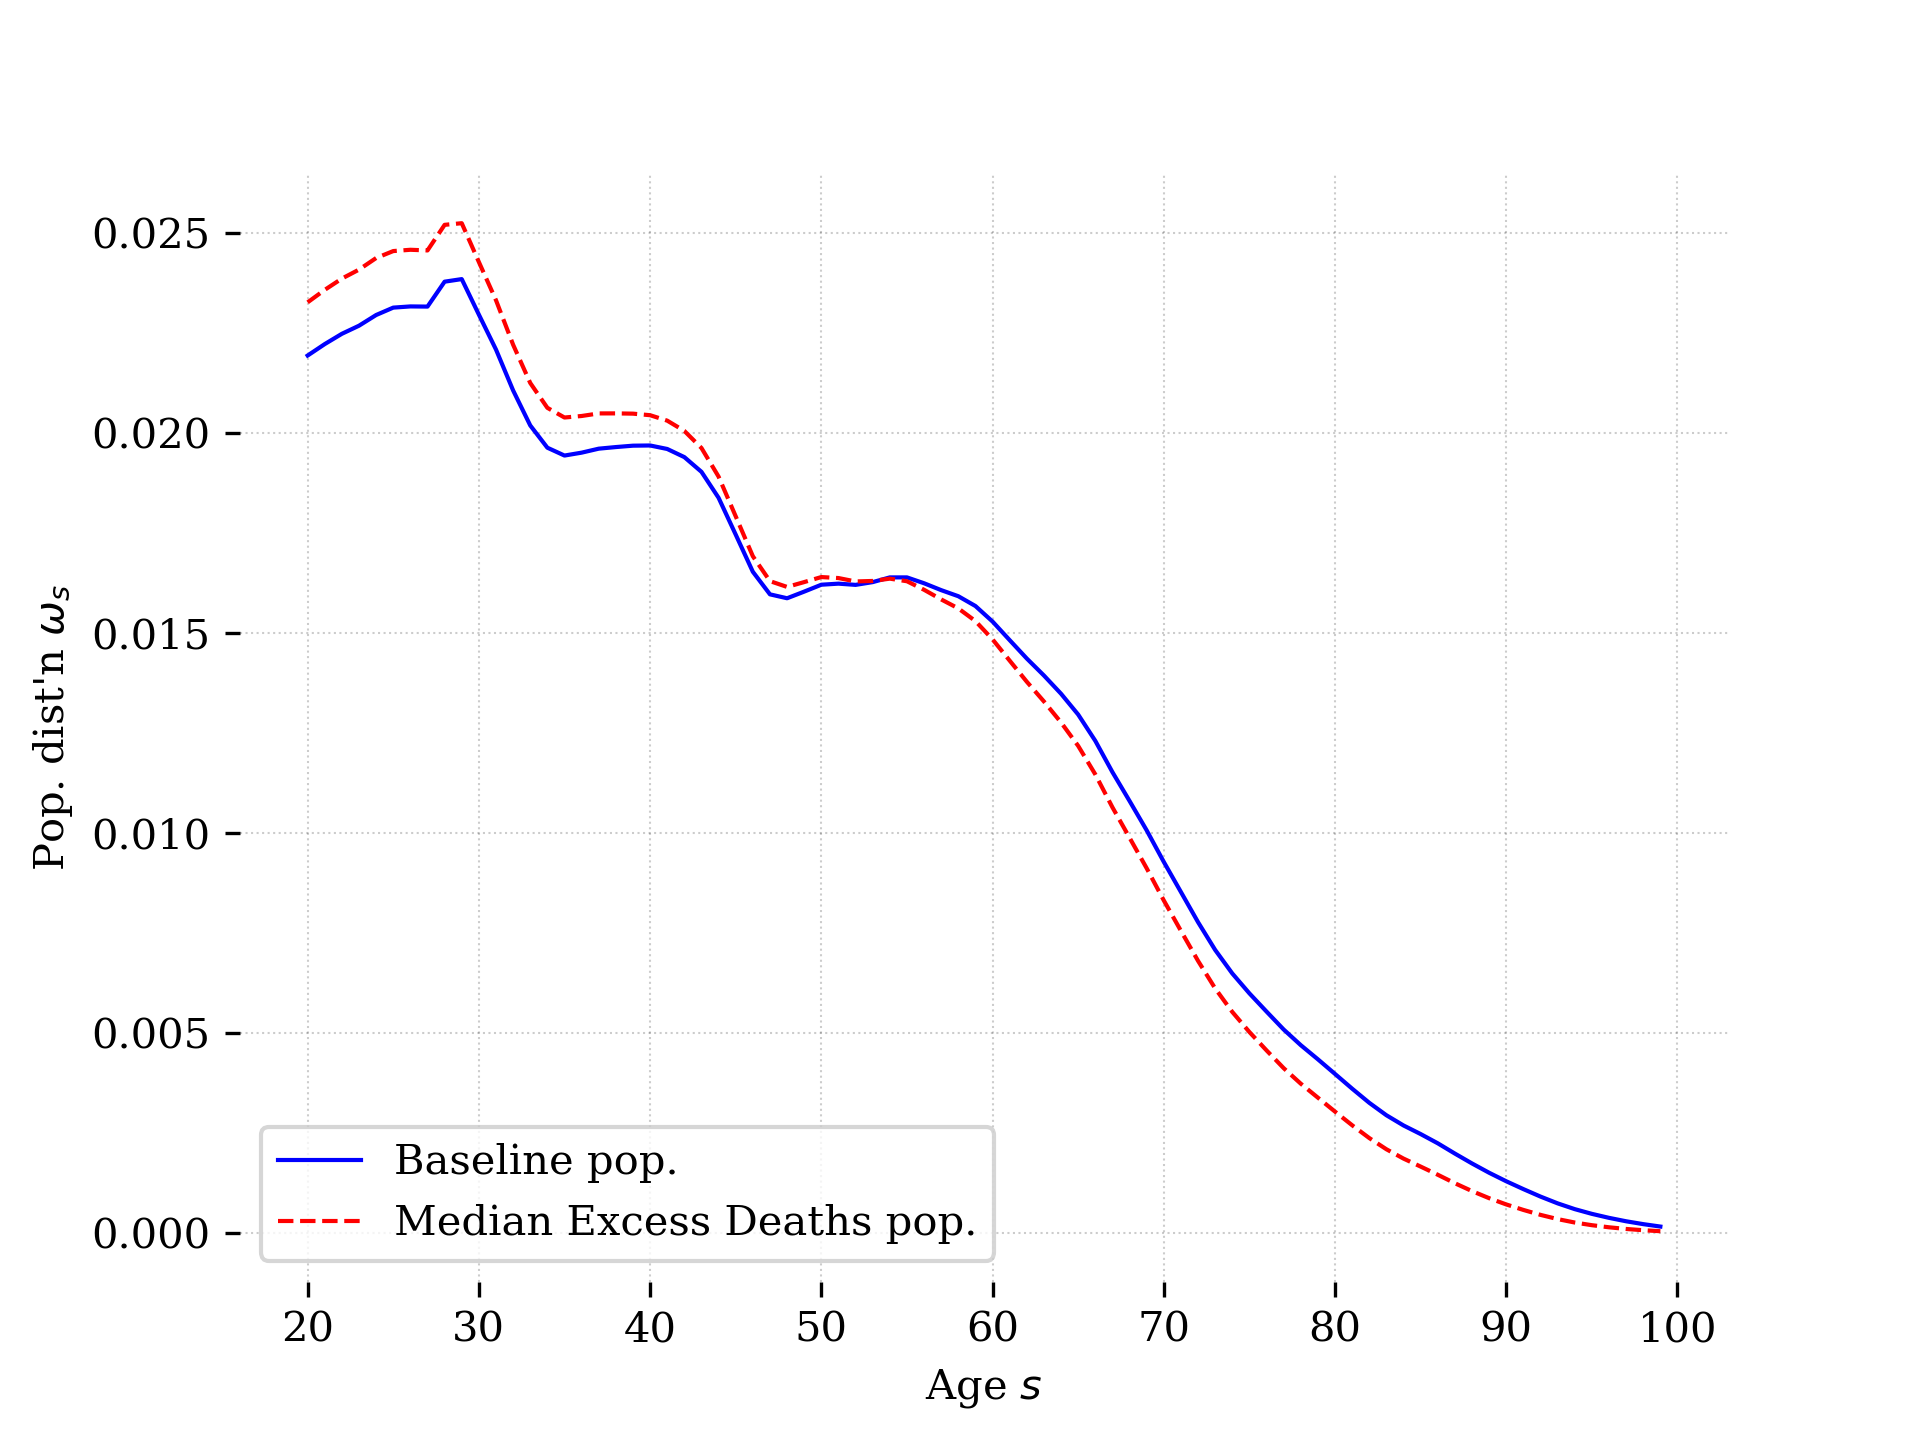
\includegraphics[scale=0.75]{./tables_figures/pop_dist_2050.png}
% \end{figure}



\subsection{Absenteeism and labor force participation}

To simulate the economic impact of disease-related morbidity among working-age individuals we impose an adjustment that reflects the effects on worker availability and productivity. This is a key margin of economic vulnerability in the absence of continued treatment and labor market support for people affected with HIV and tuberculosis.

The HIV-related productivity shock is grounded in the International Labour Office (ILO) global estimates of the economic impact of AIDS \citep{ILO2018}. That methodology distinguishes between several channels through which HIV affects the labor market: (1) premature mortality, (2) reduced productivity among HIV-positive individuals who remain employed, (3) absenteeism due to illness or caregiving responsibilities, and (4) turnover and retraining costs. The first channel is captured using our mortality scenarios described above, while this section focuses on the productivity losses due to absenteeism and partial labor force withdrawal.

ILO data for South Africa from 2005 to 2020 show a sharp decline in the number of individuals partially or fully unable to work due to HIV---from over 163,000 in 2005 to fewer than 2,300 in 2020. This decline reflects improved access to antiretroviral therapy and greater inclusion of HIV-positive individuals in the labor market. As a share of the working-age population (ages 15--64), total absenteeism fell from approximately 0.52\% in 2005 to just 0.006\% in 2020. In our simulation, we assume a reversal of these gains, returning to the 2005 level of absenteeism. The rate of absenteeism due to HIV is calculated as:
\[
\textit{absenteeism} = (\textit{partial share} \times \textit{impairment rate}) + \textit{full share}
\]
In 2005, the partial and full shares were 0.35\% and 0.17\%, respectively. We apply the ILO’s ``high impact'' scenario for the impairment rate, which assumes a 55\% productivity loss for those partially unable to work \citep{ILO2018}. This yields a total absenteeism rate of 0.361\%.

For tuberculosis, we apply an additional uniform labor supply penalty based on South Africa's 2023 TB incidence by age and empirical estimates of productivity loss from \citet{Keogh2024}, which studied the impact of TB on work absences in India. The estimate assumes a high-impact scenario in which each TB case results in a 14.4\% impact on work absences.\footnote{The paper estimates a 17.3\% increase on absences, which is then adjusted to reflect a 6-day workweek in the Indian context. The result is a 14.4\% impact} We apply this absenteeism rate to the total share of the working-age population (ages 15 and above) with current and additional TB cases. To isolate the net impact, we subtract the baseline productivity loss—calculated by applying the low-impact scenario to current TB cases—from the total productivity loss under the high-impact scenario applied to all TB cases. This yields a net TB-related adjustment of 0.0276\%, which is held constant over the simulation horizon.

The HIV-related and TB-related productivity shocks are combined to produce a total annual labor supply penalty of 0.388\% (0.361\% + 0.0276\%). This value adjusts the labor disutility parameter in the model and is applied uniformly to the bottom 70\% of the skill distribution among working-age individuals (ages 20–64), reflecting greater vulnerability to untreated illness in lower-income populations.\footnote{This is the $\chi^n_s$ described in the OG-Core model documentation and reflects the relative value of leisure versus consumption in the household's utility function.} Applying these changes to only the bottom percentiles is intended to reflect the lower access to additional healthcare resources among this group and thus lowered ability to treat the chronic effects of disease that lead to lower labor force participation. The changes are held constant throughout the simulation to reflect persistent productivity losses in the absence of expanded care. The changes in the disutility of labor result in declines in labor force participation as we expect from increased disease prevalence.

We apply the 0.388\% adjustment in our mid-range scenario, while the low- and high-impact scenarios apply adjustments equal to 50\% and 150\% of this value, resulting in 0.194\% and 0.582\%, respectively. Table \ref{tab:scenarios} presents a summary of each scenario parameters.


\begin{table}[H]
\centering
\caption{Summary of Mortality and Absenteeism Assumptions by Scenario}
\label{tab:scenarios}
\begin{tabular}{lccl}
\toprule
Scenario & \shortstack{Study} & \shortstack{Excess deaths \\ {(annual)}} & \shortstack{Absenteeism Impact} \\
\midrule
Low     & \citet{Brink2025}   & 98,350    & 0.194\% (50\% of baseline) \\
Medium  & \citet{Gandhi2025}  & 132,600   & 0.388\% (baseline) \\
High    & \citet{KS2025}      & 192,212   & 0.582\% (150\% of baseline) \\
\bottomrule
\end{tabular}
\end{table}


\section{The Economic Costs of Disease}\label{SecResults}

We simulate each of the three scenarios described above with the aforementioned adjustments to mortality and household disutility of work. The simulation results show that the macroeconomic costs of a resurgence of disease in South Africa from US aid cuts are substantial and persistent. These costs arise from sustained increases in mortality and reductions in labor force participation following the abrupt cessation of external health funding.

Table \ref{tab:avgGDPChange} presents the average annual GDP losses over the first 20 years of the simulation horizon. In the medium scenario, our preferred specification, South Africa's GDP declines by approximately \$14.8 billion per year (in 2025 USD), or about 3.5\% of GDP. Under the low excess deaths scenario, the annual loss is about \$11 billion, while in the high excess deaths scenario, the average annual GDP loss approaches \$21 billion. These losses reflect persistent reductions in effective labor supply and human capital accumulation. Recall that total global US development assistance for health was about \$21 billion in 2021, about the same as the average annual GDP loss in the high excess death scenario. If we compare these average annual reductions in GDP to US health assistance to South Africa only, which was \$462 million in 2023, the benefit to cost ratio would be about 22 to 1 in the low excess death scenario (lost GDP of \$11B to assistance of \$0.5B).\footnote{See \href{https://foreignassistance.gov}{https://foreignassistance.gov}.} We also note that GDP impacts of disease are a very narrow measure of the true benefits to society of disease prevention.  Therefore, our estimates should be thought of as the most conservative way to think about the costs of increased disease prevalence. However, even with this strict metric, the costs-benefit ratio heavily favors the side of continued support for health systems in South Africa.

\begin{table}[H] \centering \captionsetup{width=6.0in}
  \caption{\label{tab:avgGDPChange}Average Annual South African GDP Change over 20 Years}
  \begin{tabular}{llcc}
    \hline\hline
             &       & Excess deaths & Avg. annual $\Delta$ GDP \\[-1.5mm]
    \multicolumn{1}{c}{Scenario} & \multicolumn{1}{c}{Study} & (annual) & (2025\$ billions) \\
    \hline\hline
    Low    & \citet{Brink2025}  &  98,350 & -10.88 \\
    Medium & \citet{Gandhi2025} & 132,600 & -14.80 \\
    High   & \citet{KS2025}     & 192,212 & -20.81 \\
    \hline\hline
  \end{tabular}
\end{table}

Table \ref{tab:NPVLosses} summarizes the net present value (NPV) of cumulative GDP losses under each scenario, with each row representing a difference discount rate used for the NPV calculation. In the medium scenario using a 2\% discount rate (second row, third column), the total discounted loss amounts to over \$1.4 trillion (in 2025 USD). The low scenario yields an NPV loss of \$525 billion, while the high scenario projects losses exceeding \$2.9 trillion. These values highlight the long-run macroeconomic consequences of disruptions to disease control and treatment services. To compare these economics costs to the cost of prevention, we can take the amount of foreign assistance for health programs in South Africa before 2025 and assume this support would continue indefinitely. This assistance totaled about \$500 million per year.\footnote{See \href{https://foreignassistance.gov}{https://foreignassistance.gov}.} The NPV (at a 2\% discount rate) of providing this level of funding in perpetuity is \$25 billion. So as a direct comparison, the NPV of the economic costs of disease (\$1.4 trillion) is 56 times larger than the cost of prevention (\$25 billion).

\begin{table}[H] \centering \captionsetup{width=6.0in}
  \caption{\label{tab:NPVLosses}Net Present Value of GDP Loss (billions of 2025 USD)}
  \begin{tabular}{lrrr}
    \hline\hline
    Discount & Low scenario & Medium scenario & High scenario \\[-1.5mm]
    rate & \citet{Brink2025} & \citet{Gandhi2025} & \citet{KS2025} \\
    \hline\hline
    1\% & -447.83 & -2,170.70 & -5,017.78 \\
    2\% & -525.35 & -1,428.99 & -2,917.75 \\
    3\% & -472.10 & -979.31 & -1,811.36 \\
    4\% & -391.20 & -696.53 & -1,194.60 \\
    6\% & -253.34 & -387.97 & -604.44 \\
    \hline\hline
  \end{tabular}
\end{table}

These results indicate that the economic burden of disease extends far beyond the direct costs to the health sector. Even in the more optimistic scenario, where the health system absorbs much of the shock, the loss in output is substantial. The high-impact scenario shows that a collapse in treatment access and mitigation capacity could result in GDP losses equivalent to 5.5\% of South Africa's GDP.

% NOTE: SA GDP in USD in 2023 was 380 billion.


\section{Conclusion}\label{SecConc}

This analysis shows that the economic costs of a resurgence in disease following the abrupt withdrawal of external health aid are both large and persistent. In South Africa, the medium scenario---grounded in epidemiological projections and labor market data---suggests net present value GDP losses of over \$1.4 trillion USD. Even in the most optimistic case, estimated losses exceed \$525 billion in net present value. In the high-impact scenario, losses top \$2.9 trillion, over 56 times the amount of pre-2025 US health assistance to South Africa. Thus, losses are not only large in absolute terms; they are disproportionate relative to the funding at stake.

The economic damage stems not only from increased mortality, but also from more subtle and compounding effects: labor market withdrawal and reduced productivity.  These channels reinforce each other over time, undermining growth and worsening inequality. While the health consequences of aid withdrawal are immediate and visible, the economic consequences unfold more slowly—and are therefore at risk of being underestimated.

In the face of such large returns to economic investments in public health, one might ask why these expenditures are debated at the government level. As mentioned in the introduction, many developing countries lack the capacity to deliver the specialized infrastructure associated with public health funding. As such, it is not just a matter of cost, but also of expertise. In addition, many of the developing countries that would benefit most from public health funding are the least able to fund the expenditures required. For this reason, public health organizations should assess the potential returns, negotiate methods for delivery of services, and innovate methods to finance these expenditures.

Our results underscore the fragility of growth in settings of high disease burden and where treatment access hinges on foreign aid. They also highlight the risks of short-term budget decisions with long-term developmental consequences. Macroeconomic modeling of public health investments allows a quantitative assessment of the short-, medium-, and long-run costs and benefits of these investments.


\end{spacing}

\section*{Data availability}

All Python code and documentation for the computational examples and analyses are available at \href{https://github.com/OpenSourceEcon/CostOfDisease}{https://github.com/OpenSourceEcon/CostOfDisease}.
\bibliography{disease.bib}


\end{document}
